 \documentclass[rgb, pdf]{beamer}
\usepackage{listings}
\usepackage[algoruled,boxed,vlined]{algorithm2e}
\makeatletter 
\g@addto@macro{\@algocf@init}{\SetKwInOut{Parameters}{Parameters}} 
\makeatother
\newcommand{\hrulealg}[0]{\vspace{1mm} \hrule \vspace{1mm}}


\usetheme{Konstanz}
\format{169}

\title{Thesis Proposal Summary}
\titleCorporateDesign{Thesis}{Proposal}{Summary}{}
\author{Fabian Klopfer}
\date{\today}
\institute{Modelling of Complex Self-Organizing Systems Group}

\bibliography{resources}
\renewcommand*{\bibfont}{\tiny}

\begin{document}
    \usebeamerfont{normalfont}
    \begin{frame}
        \titlepage
    \end{frame}

    \begin{frame}{Introduction}
        In the last presentation $\dots$ \\ \vspace{0.5cm}
        \begin{itemize}
            \item introduced CRNs \& ODEs \\ \vspace{0.7cm}
            \item looked at Tribastone et al.~\autocite{Cardelli2017MaximalAO} \\ \vspace{0.7cm}
            \item compared the algorithms informally \\ \vspace{0.7cm}
            \item tried to find representations between CRNs \& WAs \\ \vspace{0.7cm}
        \end{itemize}
    \end{frame}
    
    \begin{frame}{What we discussed then}
        \begin{itemize}
            \item Look at classical lumping rather than CRN species lumping \\  \vspace{0.7cm}
            \item Construct ``middle ground'' between WAs \& CTMCs using fully probabilistic Segala \\ \vspace{0.7cm}
            \item Elaborate on connection between Kiefer~\autocite{Kiefer2013OnTC} and partition refinement-based lumping e.g. Valmari et al.~\autocite{valmari} \\ \vspace{0.7cm}
        \end{itemize}
    \end{frame}
   
    \begin{frame}[allowframebreaks]{Schützenberger's construction \& Bisimulation}
       Schützenberger~\autocite{schutz} vs. Buchholz~\autocite{buchholz2008bisimulation}: 
        \begin{align}
         \overrightarrow{\mu}(\sigma) & = \overrightarrow{F} \mu(\sigma) \overrightarrow{F}^{-1}_R 
         & \overrightarrow{F} \mu(\sigma) & = \overrightarrow{\mu}(\sigma)\overrightarrow{F} \\
       \hat{P} & = W P V & W P & = \hat{P} V_R^{-1} 
        \end{align}   With $W \cdot V = I$ and $P$ the transition matrix. \\
        \vspace{0.7cm}
        \[ W \cdot V = I \]
        \[ W \cdot V \cdot V^{-1}_R = I \cdot V^{-1}_R \]
        \[ W = V^{-1}_R \]
        Thus we get 
        \begin{align}
         \overrightarrow{\mu}(\sigma) & = \overrightarrow{F} \mu(\sigma) \overrightarrow{F}^{-1}_R 
         & \overrightarrow{F} \mu(\sigma) & = \overrightarrow{\mu}(\sigma)\overrightarrow{F} \\
       \hat{P} & = W P W^{-1}_R & W P & = \hat{P} W
        \end{align}
        \end{frame}
        
        \begin{frame}[allowframebreaks]{WA $\leftrightarrow$ labelled CTMC}
        WA $\leftrightarrow$ CTMC: A labelled CTMC is already a WA. \\ scale WA by row sum per row and letter to get (sort of) a labeled DTMC which can be interpreted as uniformized labelled CTMC (sort of).
        \framebreak
        
        Problem: Only one labelled transition possible per state. \\
        
        What we get is actually not a MC but rather a deterministic Rabin PA. \\
        
        \begin{center}
        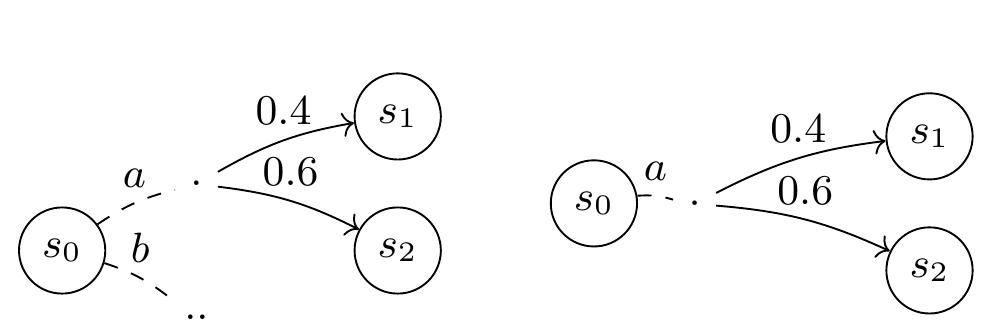
\includegraphics[keepaspectratio, height=0.4\textheight]{img/lmc_rpa}
        \end{center}    
        
           $\Rightarrow$
         A \textbf{WA} may be normalized by left. mult. vector of sum of row sums, yielding a \textbf{f.p. Segala}, i.e. the row sum of all matrices together equals 1. \\ 
         Drop the labels of the \textbf{f.p. Segala} and add the matrices together to get a \textbf{DTMC}, which can be viewed as \textbf{uniformized CTMC}. \\ \vspace{1.4cm}
         
         $\Leftarrow$
         A \textbf{CTMC} can be uniformized to a \textbf{DTMC}. Scaling each probability by the number of letters yields a \textbf{f.p. Segala}, which is already a \textbf{WA}\\ \vspace{1.4cm}
         
         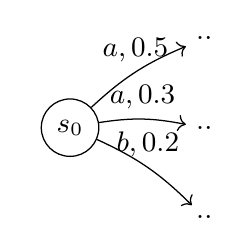
\includegraphics[keepaspectratio, height=0.4\textheight]{img/fps}
         
         Problem: Paths \& Probabilities are preserved but what are the labels?
         \framebreak
         
         Labelled CTMC is already a WA.\\
         
         WA $\rightarrow$ CTMC: Resort to the following:
            \begin{enumerate}
             \item Generate the language, i.e. all weights with all words
             \item for every word build a LCTMC with the adequate labels and all transition probabilities set to 1.
             \item sum the weights for all words.
             \item connect all generated LCTMCs to an extra state, add an extra empty label transition matrix with transitions from extra state to respective word with probability $\frac{\text{word weight}}{\text{weight sum}}$
            \end{enumerate}

        \end{frame}

    
    \begin{frame}[allowframebreaks]{Connection between the algorithms}
         Weighted automaton $\mathcal{A} = (n, \Sigma, \mu, \alpha, \eta)$ with \\ \vspace{0.5cm}
            \begin{minipage}{0.27\textwidth}
                \begin{itemize}
                    \item $n = 3$,
                    \item $\Sigma = \{a, b\}$,
                    \item $\alpha = (\alpha_0,\alpha_1, \alpha_2, \alpha_3)$,
                    \item $\eta = (\eta_0,\eta_1, \eta_2, \eta_3)$,
                \end{itemize}
            \end{minipage} \begin{minipage}{0.28\textwidth}
             \begin{itemize}
                 \item $\mu(a) = \begin{pmatrix}
                                    0 & \frac{1}{2} & \frac{1}{2} & 0 \\
                                    0 & 0 & 0 & 0 \\
                                    0 & 0 & 0 & 0 \\
                                    0 & 0 & 0 & 0
                                \end{pmatrix}$, \vspace{0.2cm} \\
                    \item $\mu(b)= \begin{pmatrix}
                                    0 & 0 & 0 & 0 \\
                                    0 & 0 & 0 & 1 \\
                                    0 & 0 & 0 & 1 \\
                                    0 & 0 & 0 & 0
                                 \end{pmatrix}
                                $.
                \end{itemize}
            \end{minipage}
            \begin{minipage}{0.3\textwidth}
            \begin{center}
                \begin{tikzpicture}[shorten >=1pt,node distance=2cm,on grid,auto] 
                    \node[state,initial] (z_0)   {$z_0$}; 
                    \node[state] (z_1) [above right=of z_0] {$z_1$}; 
                    \node[state] (z_2) [below right=of z_0] {$z_2$}; 
                    \node[state](z_3) [below right=of z_1] {$z_3$};
                        \path[->] 
                        (z_0) edge  node {a/$\frac{1}{2}$} (z_1)
                            edge  node [swap] {a/$\frac{1}{2}$} (z_2)
                        (z_1) edge  node  {b/1} (z_3)
                        (z_2) edge  node [swap] {b/1} (z_3);
                \end{tikzpicture}
            \end{center}
            \end{minipage}
            
            \framebreak
            
            \[  \mu(a)^2 = (0);  \ \ \mu(b)^2 = (0); \ \ \mu(b) \mu(a) = 0  \]
            $\Rightarrow$ Words to consider: a, b, ab
            
            
            \[  r^{(i)}= \begin{pmatrix}
                        r^{(i)}_{a,0} & r^{(i)}_{a,1} & r^{(i)}_{a,2} & r^{(i)}_{a,3} \\
                        r^{(i)}_{b,0} & r^{(i)}_{b,1} & r^{(i)}_{b,2} & r^{(i)}_{b,3}
                    \end{pmatrix}                     
        \] \vspace{0.5cm}
        \[ v_i = \alpha \mu(a) r^{(i)}_a + \alpha \mu(b) r^{(i)}_b + \alpha \mu(a) \mu(b) r^{(i)}_{ab} \]
        \[= \left(0, \frac{1}{2} \alpha_0, \frac{1}{2} \alpha_0, 0\right) r^{(i)}_a + \left(0, 0, 0,\alpha_1 + \alpha_2\right) r^{(i)}_b + \left(0,0,0,\alpha_0\right) r^{(i)}_{ab} \]
        \[ = \left(0, \frac{1}{2} r^{(i)}_{a,0} \alpha_0, \frac{1}{2} r^{(i)}_{a,0} \alpha_0, r^{(i)}_{b,0} [\alpha_1 + \alpha_2] + r^{(i)}_{a,0} r^{(i)}_{b,1} [\alpha_0] \right) \]
        
         \[ \overrightarrow{F} = \begin{pmatrix}
                                    \alpha_0 & \alpha_1 & \alpha_2 & \alpha_3 \\
                                    0 & \frac{1}{2} r^{(1)}_{a,0} \alpha_0 & \frac{1}{2} r^{(1)}_{a,0} \alpha_0 & r^{(1)}_{b,0} [\alpha_1 + \alpha_2] + r^{(1)}_{a,0} r^{(1)}_{b,1} [\alpha_0]   \\
                                    0 & \frac{1}{2} r^{(2)}_{a,0} \alpha_0 & \frac{1}{2} r^{(2)}_{a,0} \alpha_0 & r^{(2)}_{b,0} [\alpha_1 + \alpha_2] + r^{(2)}_{a,0} r^{(2)}_{b,1} [\alpha_0]   \\
                                \end{pmatrix}
        \] \\ \vspace{0.6cm}
        Using partition refinement we get $\{s_1, s_2\}$, thus \[ W = \begin{pmatrix}
                                    1 & 0 & 0 & 0 \\
                                    0 & \frac{1}{2} & \frac{1}{2} & 0 \\
                                    0 & 0 & 0 & 1
                                \end{pmatrix} \]\\
                                \framebreak
                                
        Chose $\alpha = (1,0,0,0)$. \\
        Now Kiefer restricts the $r^{(i)}_{\sigma,k}$ to $\mathbb{N_+}$. \\
        Resulting in that it is not possible to find parameters such that $\overrightarrow{F} = W$. \\
        Even when we loosen that restriction, chose $r^{(1)}_{a,0} = 1, r^{(1)}_{b,0} = r^{(1)}_{b,1} = 0, r^{(2)}_{a,0} = 0, r^{(2)}_{b,0} = 1$.\\
        Still impossible as $\overrightarrow{F}{i=j=4} \new 1$. \\
        \end{frame}
        
        \begin{frame}[allowframebreaks]{Summary}
        \begin{itemize}
         \item Kiefers et al.~\autocite{Kiefer2013OnTC} basis construction not able to produce the same basis as partition refinement
         \item yields non-sparse transition matrices 
         \item induces computational overhead, possibly more overhead than gaining by dimensionality reduction
         \item Alternative: Use Householder reflectors for finding the basis~\autocite{kieferstab}, yield potentially sparser transition matrices while numerically stable wo. hacks
         \item Partition-refinement does \textbf{not} explicitly construct a basis.
         \item rather constructs new  transition matrix than transforming old one
        \end{itemize}
        \framebreak
         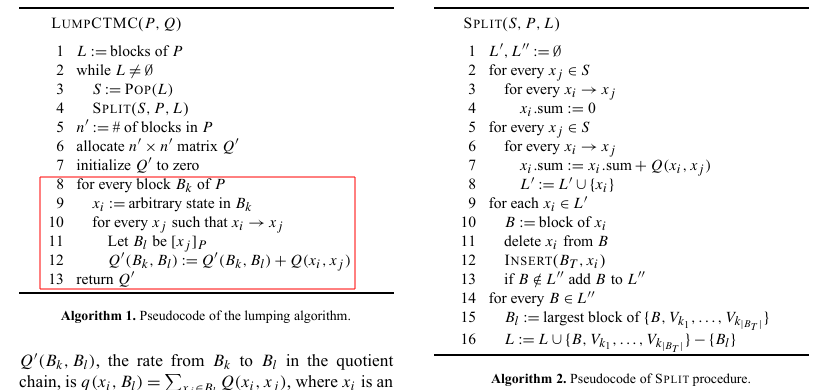
\includegraphics[height=0.8\textheight, width=\textwidth, keepaspectratio]{img/derisavi_pseudocode.png}
    \end{frame}

    \begin{frame}{Bibliography}
        \printbibliography
    \end{frame}
\end{document}
